\newchapstyle
\chapter{Introduction}
\label{chap:intro}

%\epigraph[0pt]{
%    Failure is not an option.
%}{Actor Ed Harris, playing flight director Gene Kranz, in the 1995 film Apollo 13\cite{FailureNotOption2019}}

%\begin{abstract}
%Lorem ipsum dolor sit amet, consectetur adipisicing elit, sed do eiusmod tempor incididunt ut labore et dolore magna aliqua. Ut enim ad minim veniam, quis nostrud exercitation ullamco laboris nisi ut aliquip ex ea commodo consequat. Duis aute irure dolor in reprehenderit in voluptate velit esse cillum dolore eu fugiat nulla pariatur. Excepteur sint occaecat cupidatat non proident, sunt in culpa qui officia deserunt mollit anim id est laborum.
%\end{abstract}

%% Start the actual chapter on a new page.
\afterpage{\pagecolor{none}}\newpage

\section{Superconducting-normal Josephson devices}

\subsection{Andreev reflection and Andreev bound states}

The process of Andreev reflection at the interface between superconductors and normal metals lays the fundament for understanding how a Josephson junction works.
%
The process is sketched in Fig. \ref{fig:kdtmk}:
%
An electron impinging onto the super-normal interface from inside the normal region can only enter the superconductor in the form of a Cooper pair by being reflected as a hole with opposite spin and momentum.
%
Vice versa, a Cooper pair travelling towards the normal region will decay into an electron travelling forward, and annihilate a hole travelling backwards with spin opposite to that of the electron.
%
Inside the normal region, this will result in the formation of the so-called Andreev bound states (ABS).

Since inside the superconductor, there are no states allowed for $\epsilon_F - \Delta \leq \epsilon_F \leq \epsilon_F - \Delta$, the superconducting electrodes can be though of as forming potential barriers at the interface, leading to transparencies $\tau$, and the Andreev paris can be thought of analogously as particles inside a box.
%
Here also elaborate on the Thouless energy and 2D junctions.

Nanda \textit{et al.}~\cite{nandaCurrentPhaseRelationBallistic2017} point out an important factor to take into account:
%
Skewness can quite significantly depend on the S-N interface, i.e. transparency, and the ratio $L/\xi$.
%
Temperature additionally suppresses skewness, since this leads to a higher number of quasiparticles, and increases the amount of continuum states contributing to the supercurrent.

\begin{align}
\frac{\partial\delta}{\partial t}&=\frac{2eV_J}{\hbar}\, ,\, V_J=L_J\frac{\partial I_J}{\partial t}=L_J\frac{\partial I_J}{\partial\delta}\frac{\partial\delta}{\partial t}
\end{align}

The work done on the junction must be $U_J=\int I_J V_J {\rm d}t=\frac{\hbar}{2e}\int I_J \frac{\partial\delta}{\partial t}{\rm d}t = \frac{\hbar}{2e}\int I_J {\rm d}\delta$, therefore $I(\delta) = \frac{2e}{\hbar}\frac{\partial U_J}{\partial\delta}$.
Each Andreev bound state has a ground state energy $U_i=-\Delta\sqrt{1-T_i\sin^2(\delta/2)}$ with induced superconducting gap $\Delta$ and channel transparency $T_i$.
Summing over all of these channels, the total Josephson potential is given by
\begin{align}
U_J(\delta) &= 1-\Delta\sum_i\sqrt{1-T_i\sin^2(\delta/2)} \\
&\approx E_J \frac{\delta^2}{2} - E_J\left( 1-\frac{3\sum T_i^2}{4\sum T_i} \right) \frac{\delta^4}{24} +\mathcal{O}(\delta^6)\ , \\
E_J &= \frac{\Delta}{4}\sum_i T_i \rightarrow \frac{\Delta}{4}N\tau
\end{align}

The corresponding Josephson current and inductance are 
\begin{align}
I(\delta) &= \frac{2e}{\hbar}\frac{\partial U_J}{\partial\delta} = \frac{e\Delta}{2\hbar}\frac{\tau\sin\delta}{\sqrt{1-\tau\sin^2\delta/2}} \\
L_J(\delta) &= \frac{\hbar}{2e}\left( \frac{\partial I_J}{\partial\delta} \right)^{-1} = \left(\frac{\hbar}{2e}\right)^2\left(\frac{\partial^2U_J}{\partial\delta^2}\right)^{-1}
\end{align}

\begin{figure}
	\centering
	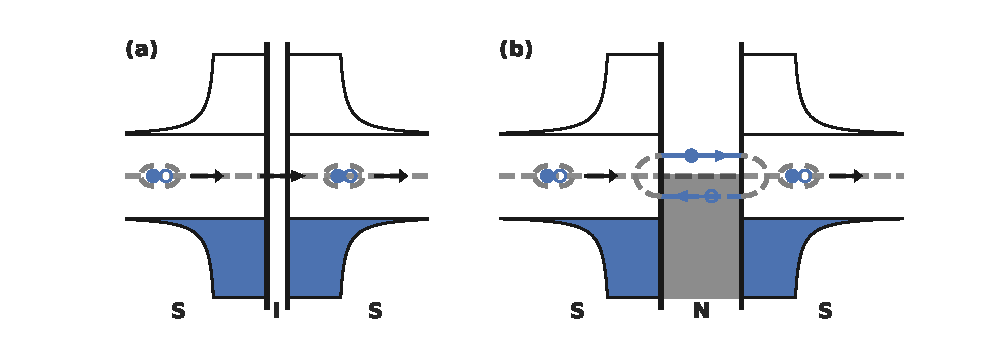
\includegraphics[width=\linewidth]{chapter-introduction/figs/model_SNS_DOS}
	\caption{
		\textbf{Cooper pair transport in SIS and SNS Josephson junctions.}
		%
		The density of states in a superconductor exhibits a gap of width $2\Delta$ in energy around the Fermi level $\epsilon_F$, with states below $\epsilon_F$ filled and states above unoccupied.
		%
		\textbf{(a)} In an SIS Josephson junction, Cooper pairs, consisting of an electron and hole with opposite spins can tunnel through a thin insulating barrier separating two superconducting banks.
		%
		There are no states inside the insulating region.
		%
		\textbf{(b)} In an SNS Josephson junction, the normal region exhibits a DOS that is filled up to $\epsilon_F$.
		%
		Cooper pairs entering the normal region are broken up into electrons and holes of opposite spin and momentum, that can enter the superconductor under Andreev reflection, thus forming Andreev bound states within the normal region.
		%
		This results in a net current across the junction.
	}
	\label{fig:modelsnsdos}
\end{figure}

\begin{figure}
	\centering
	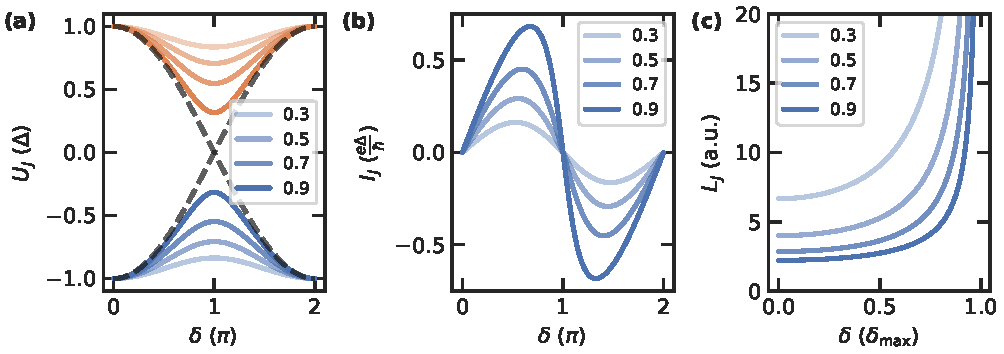
\includegraphics[width=\linewidth]{chapter-introduction/figs/model_SNS_EjIc}
	\caption{
		\textbf{Channel transmission and nonsinusoidality.}
		%
		\textbf{(a)} Josephson energy of the ground (blue) and excited (orange) Andreev bound state for varying channel transmission $\tau$ as a function of phase drop across the Josephson junction.
		%
		Increasing color intensity corresponds to increasing $\tau$.
		%
		Dashed line corresponds to $\tau=1$.
		%
		\textbf{(b)} Josephson current for varying $\tau$.
		%
		Increasing transmission increases both amplitude and forward skewing of the CPR.
		%
		\textbf{(c)} Josephson inductance as a function of phase normalized to the one at maximum $L_J$.
		%
		Due to the increased CPR slope for increasing $\tau$ at zero phase, the Josephson inductance decreases.
	}
	\label{fig:modelsnsejic}
\end{figure}


The anharmonicity in the circuit is then reduced depending on the channel transparencies.
In the limit of small $L_J$, we can model the TL resonator as a series $LC$-circuit, resulting in anharmonicity
\begin{align}
\chi &= \frac{-E_C}{2} \left( 1-\frac{3\sum T_i^2}{4\sum T_i} \right) p^3 \rightarrow \frac{-E_C}{2} \left(1-\frac{3}{4}N\tau \right) p^3 
\end{align}


\subsection{Subgap density of states}

KWANT~\cite{grothKwantSoftwarePackage2014} simulations are at \url{https://nas-steelelab.tnw.tudelft.nl:5001/?launchApp=SYNO.SDS.Drive.Application#file_id=509401234564752146}, located on the NAS under \texttt{Felix/programming/kwant}.

\subsection{The limit of low $\tau$: SIS}



\section{DC bias cavities for probing Josephson junctions}

%\subsection{Coplanar waveguide electrodynamics}

%\subsection{DC bias cavities}

In order to probe the Josephson inductance, we make use of superconducting microwave resonators based on coplanar waveguides~\cite{gopplCoplanarWaveguideResonators2008,zmuidzinasSuperconductingMicroresonatorsPhysics2012}.
%
These have been used extensively in the field of particle detection and circuit (quantum) electrodynamics due to the intrinsic low loss originating from the absence in resistance of the Cooper pairs~\cite{dayBroadbandSuperconductingDetector2003a,blaisCavityQuantumElectrodynamics2004c}.
%
In order to analyze our devices both in the low and high frequency range (DC to several $\SI{e9}{\hertz}$), our circuits need to be able to sustain relatively large quality factors while being able to introduce direct current and voltage access to the device under test (DUT).

While there is a variety of circuit architectures capable of this approach, such as using inductive coupling~\cite{vissersFrequencytunableSuperconductingResonators2015b}, direct leads at voltage nodes of a $\lambda/2$ resonator with matching length~\cite{chenIntroductionDcBias2011a,liApplyingDirectCurrent2013} or lumped-element split-cavities~\cite{mahashabdeFastTunableHigh2020}, we based our design on an architecture previously developed in our group, the shunt capacitor DC bias access~\cite{bosmanBroadbandArchitectureGalvanically2015c}.
%
The advantage of this approach is threefold:
%
As no circuit symmetries need to be considered, the design is rather simple.
%
No additional port needs to be used to probe or excite the DUT, thus there is no additional leakage channel.
%
Finally, using a shunt capacitor provides a broadband signal port up to the self-resonance of the shunt capacitor, which is chosen to be well above the resonance frequency of the circuit.

Figure~\ref{fig:TLmodel}(a) depicts a schematic of the DC bias cavity circuit.
%
In principle, measurements in both transmission and reflection geometry are possible.
%
However, we typically use the second port for supplying a DC gate voltage, and short the DUT to ground.
%
Therefore, we only perform reflection measurements.

The reflection coefficient of this circuit is given by
%
\begin{align}
S_{11}=-1+\frac{2\kappa_e}{\kappa_e+\kappa_i+2i\Delta}
\label{eq:intro-s11}
\end{align}
%
with the internal and external loss rates $\kappa_i$ and $\kappa_e$ and the detuning $\Delta=\omega-\omega_0$~\cite{bosmanBroadbandArchitectureGalvanically2015c}.
%
In Fig.~\ref{fig:s11} we plot the reflection coefficient for various fractions of $g_Q =\kappa_e/\kappa_i$, to illustrate the effects of over-, under- and critical coupling ($g_Q >1$, $g_Q <1$ and $g_Q =1$, respectively).
%
For a best signal-to-noise ratio, the shunt capacitor $C_s$ should be designed such that $\kappa_e=\kappa_i$, with the external loss rate approximately given by
%
\begin{align}
\kappa_e &= \frac{\omega_0}{Q_e} = \frac{2}{\pi\omega_0Z_0^2C_s^2}
\label{eq:intro-kappae}
\end{align}
%
with external quality factor $Q_e$ and transmission line impedance $Z_0$.
%
However, when placing a JJ at the end of the TL, the internal loss rate can rise significantly.
%
For this reason, we typically design our circuits such that they are overcoupled without a JJ present, anticipating a rise in $\kappa_i$.
%
As shown in the inset of Fig.~\ref{fig:s11}(a), over- or undercoupling by the same factor in fact leads to the same SNR in the absolute value of $S_{11}$.
%
It is tempting to therefore search for a circuit resonance in the measured since this provides a potentially more reliable identification method.
%
Nevertheless, measurement background from impedance mismatches, resulting in oscillations of the background, often obscure even drastic phase changes, for which reason the absolute value can at times be better suited.

\begin{figure}[t]
	\centering
	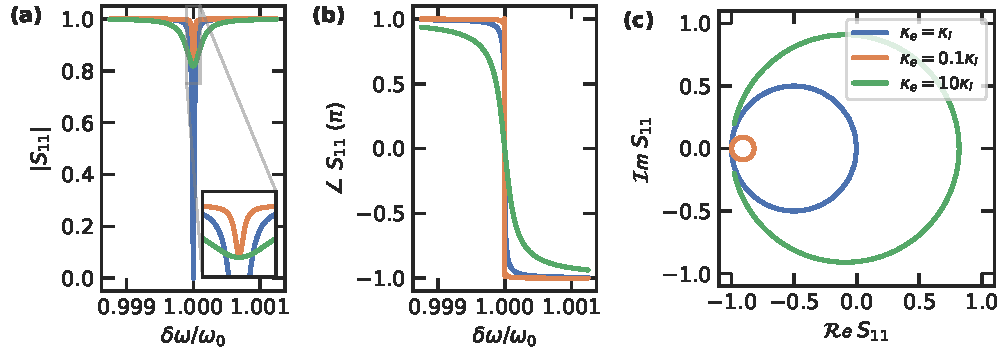
\includegraphics[width=\linewidth]{chapter-introduction/figs/model_DC_bias_cavity_coupling.pdf}
	\caption{
		\textbf{Effect of coupling ratio of the reflection coefficient of a DC bias cavity.}
		%
		Using Eq.~\ref{eq:intro-s11}, we can model the absolute value \textbf{(a)}, phase \textbf{(b)} and real and imaginary parts \textbf{(c)} of the reflection coefficient of a DC bias cavity.
		%
		Colors denote the various coupling types: blue: critically coupled $\kappa_e/\kappa_i=1$, orange: undercoupled $\kappa_e/\kappa_i=0.1$, green: overcoupled $\kappa_e/\kappa_i=10$.
		%
		Best signal-to-noise ratio is achieved for critical coupling, while the other two cases have identical SNR in terms of $\abs{S_{11}}$.
	}
	\label{fig:s11}
\end{figure}

When probing Josephson junctions with the DC bias cavity, we need to calibrate the microwave circuit parameters.
%
This is done by measuring a combination of an open and shorted reference device with the same sample geometry, except with an open or short to ground in place of the JJ.
%
Equipped with these values, we can proceed to extract information about the JJ:
%
With an added Josephson junction with inductance $L_J$ shorting the TL to ground, the shifted resonance frequency can be approximated by
%
\begin{align}
\omega_0^\prime = \omega_0\frac{L_r+L_J}{L_r+2L_J}
\label{eq:intro-omega0p}
\end{align}
%
where $L_r$ is the lumped TL resonator inductance including geometric and kinetic inductances, cf. Chapter~\ref{chap:gJJ-CPR} and Fig.~\ref{fig:TLmodel}(b).
%
A complete analytical model of an RSCJ model parametrizing the JJ can be used for calculating junction-induced losses in the form of a subgap resistance, cf. Chapter~\ref{chap:gJJ} and Fig.~\ref{fig:TLmodel}.
%
For very small $R_{\rm sg}$, the Josephson inductance is effectively short-circuited, so $Q_i$ approaches the limit of no JJ.
%
On the other hand, very large $R_{\rm sg}$ implies an open circuit with no losses other than the ones in the TL resonator, again approaching $Q_i$ of the bare cavity.
%
Intermediate resistance values suppress the resonance entirely.
%
The shift in $f_0$ for large $R_{\rm sg}$ shows the frequency shift induced by $L_J$.

\begin{figure}
	\centering
	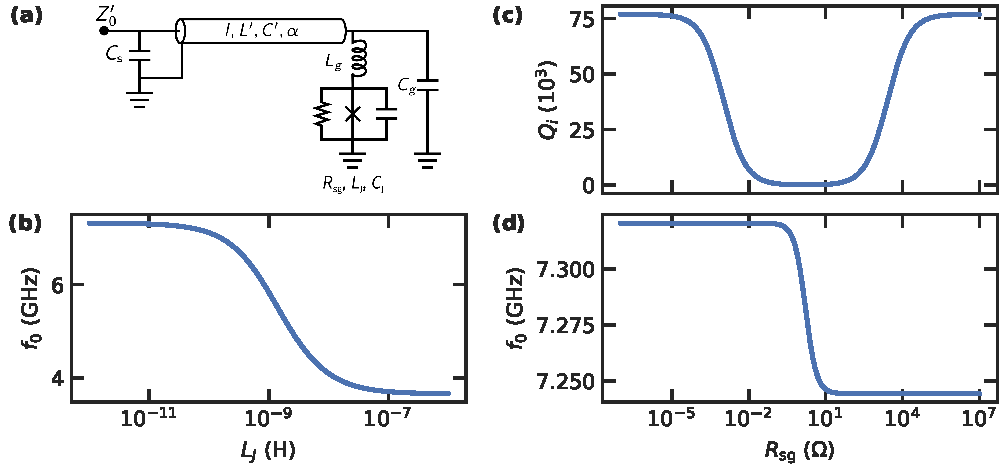
\includegraphics[width=\linewidth]{chapter-introduction/figs/model_DC_bias_cavity_params_RCSJ.pdf}
	\caption{
		\textbf{DC bias cavity shorted to ground by a parametrized top-gated graphene Josephson junction.}
		%
		\textbf{(a)} Parametrized circuit model.
		%
		\textbf{(b)} Resonance frequency versus Josephson inductance.
		%
		\textbf{(c,d)} Influence on subgap resistance on internal quality factor and resonance frequency.
		%
		Panel \textbf{(d)} also illustrates the shift of $f_0$ due to $L_J$ as in panel \textbf{(b)}.
	}
	\label{fig:TLmodel}
\end{figure}


\section{Outline}

In the following, we will show the applications of DC bias cavities to both extract information about the intrinsic parameters of the Josephson junctions to be probed, and use the combination of cavity and junction to perform a detection measurement.


In chapter~\ref{chap:experiment}, we provide a detailed overview on the experimental methods that we developed and used to enable the measurements presented later on.
%
We detail the exfoliation and fabrication of van der Waals devices, superconducting CPW resonators.
%
Additionally, a short introduction to the use of the superconducting alloy molybdenum-rhenium in Delft, together with a small study on its pros and cons, is supplied.
%
This chapter also includes a brief introduction to thermal noise and the fridge wiring used to suppress the former during measurements.

In chapter~\ref{chap:gJJ}, we present the first measurements of a graphene Josephson junction in the microwave regime.
%
Motivated by the potential use of graphene in superconducting quantum circuits, we studied the Josephson inductance by tracking the resonance frequency, and high-frequency losses of the junction attributed to its subgap resistance by extracting the added circuit losses.
%
Together with a detailed circuit characterization in both DC and the MW regime, the results indicate that graphene Josephson junctions are indeed a feasible platform for circuit quantum electrodynamics.


In chapter~\ref{chap:gJJ-CPR}, we take a closer look at the underlying mechanisms governing the Josephson inductance of graphene Josephson junctions, i.e. their current-phase relation.
%
Using previously not performed microwave measurements of DC bias cavities, we show that the CPR of diffusive and ballistic devices is forward-skewed, as is expected for these junctions.
%
We quantify the resulting correction of the Josephson energy potential, which is crucial for the use of gJJs in microwave quantum circuits.

We end the part of this thesis concerned with graphene devices with chapter~\ref{chap:gJJ-misc}.
%
Here, we provide a collection of additional DC data on graphene Josephson junctions and SQUIDs.
%
In particular, we investigate oscillations in the IV curves that occur as a result of the junction probing its electromagnetic environment in the absence, and the phase locking to the presence of microwave radiation, resulting in Fiske and Shapiro steps, respectively.


Chapter~\ref{chap:currentdetection} shows the result of a DC bias MW cavity coupled to a aluminum constriction Josephson junction.
%
Making use of the responsivity of the circuit's resonance frequency to bias current, we detect low-frequency currents with a minimum measured sensitivity of \SI{8.9}{\pico\ampere\per\hertz\tothe{1/2}}, comparable to state-of-the-art devices.
%
With an analytical circuit model, we extrapolate orders of magnitude better values for improved device designs based on our circuit, which could eventually enable quantum limited current detection.


We close with a summary of all presented results and a possible way onwards in chapter~\ref{chap:conclusion}.
%
Additional information on tips and tricks for electron beam lithography, such as alignment and height measurements, useful source code and specifications on the self-assembled low-pass and copper powder filters are appended to this thesis.


%\clearpage
%\references{dissertation}

